In this section, we will derive and apply the Onsager-Machlup path integral.
This is a formulation of Markovian stochastic processes that describe the conditional probabilities of a physical process as a sum of all possible paths the system can take
The conditional probabilities are statements of the form ``Given this intital condition, what is the probability that the system ends up here'', and the in the path integral formulation this is calculated by summing over all possible ways, or ``paths'' the system could evolve from the initial to the final state.
The physical systems that can be described by this formulation are \emph{stochastic processes.}


\section{Stochastic processes}

A stochastic process $x(t)$ is a function of $t \in \Te$, where the only requirement on $\Te$ is that it is \emph{total ordered}.
This means that, for any two elements $t_1, t_2 \in \Te$ and $t_1 \neq t_2$, then $t_1 < t_2$ or $t_2 < t_1$.
The most common example of $\Te$ is time, so $x(t)$ describes the evolution of $x$ thought time.
However, $\Te$ might also be the links in a polymer, \dots \todo{more examples?}
Furthermore, $\Te$ can be discrete or continuous.more
We will begin by considering discrete time steps with a length of $\Delta t$, so
%
\begin{align}
    \Te = \{ \dots -2 \Delta t, - \Delta t, 0, \Delta t, 2 \Delta t, \dots\} = \Delta t \Z.
\end{align}
%
The notation $\Delta t \Z$ means set of all integers $\Z$ multiplied by $\Delta t$.

We consider a stochastic process $x(t)$ that take on discrete values, $x \in \Ex$, where
%
\begin{align}
    \Ex \Delta x \Z.
\end{align}
%
This process can be though of as a particle on a one-dimensional lattice with lattice points separated by $\Delta x$.
The probability that, if the particle is at lattice point $x = n \Delta x$ at time $t$, it will jump to lattice point $x' = m \Delta x$ at the next time step $t + \Delta t$, is $P(x'(t + \Delta t) | x(t) )$.
We use there the common notation for conditional probabilities, where $P(A|B)$ means ``the probability of $A$ given $B$''.
It is defined as 
%
\begin{align}\label{eq: cond prob}
    P(A|B) P(B) = P(A\cap B),
\end{align}
%
where $P(A\cap B)$ is the probability that \emph{both} $A$ and $B$ occur.

\begin{figure}[!htb]
    \centering
    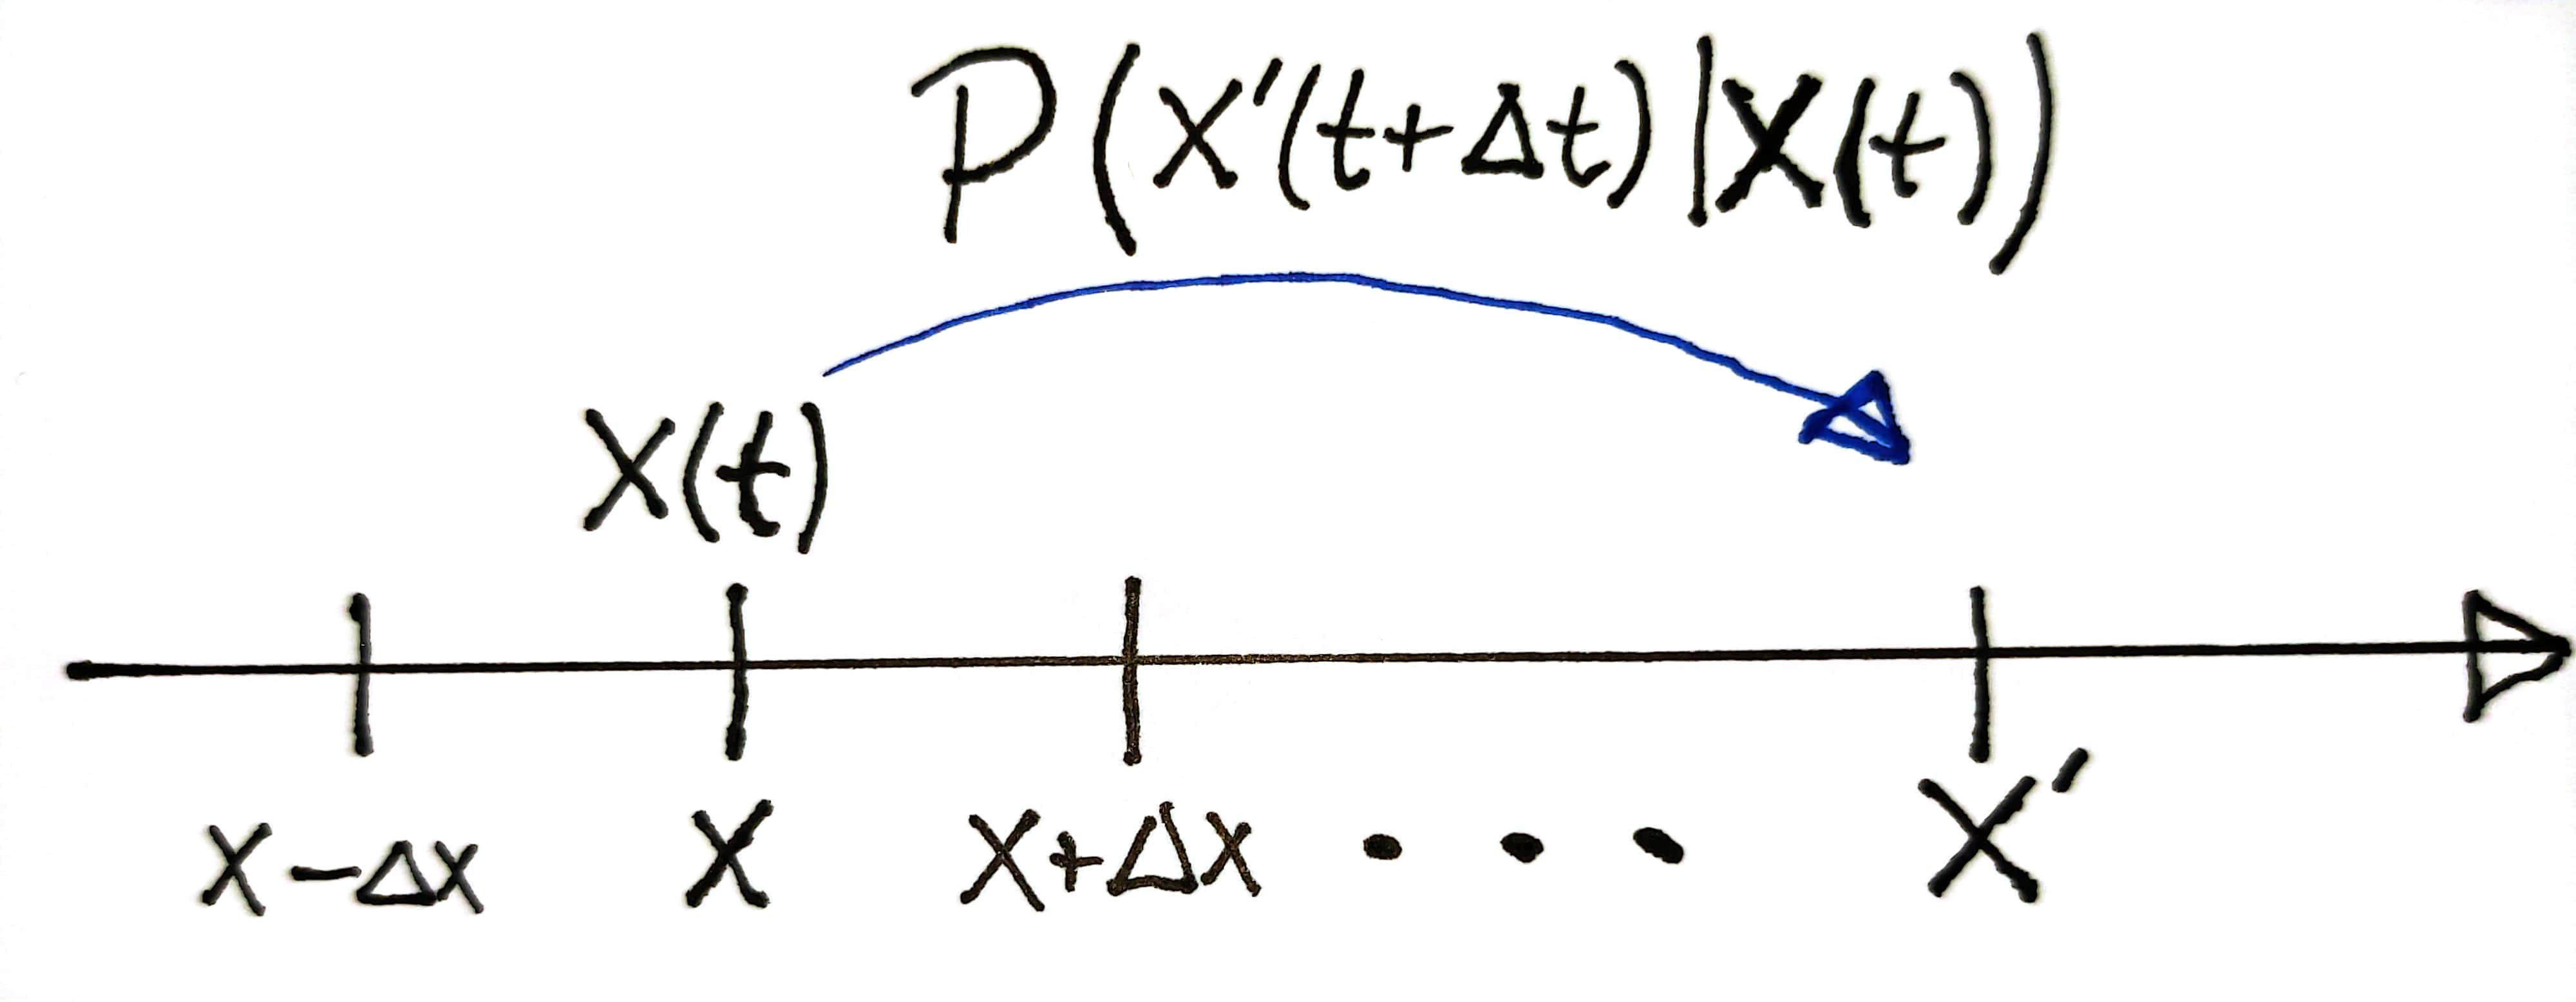
\includegraphics[width=.5\textwidth]{fig/fig1.jpg}
    \caption{Illustration of a stochastic process}
    \label{fig: stochastic process}
\end{figure}

A \emph{Markov process} is a stochastic process with ``no memory''.
This means that, if we have $n$ steps of the process $x(t_1), x(t_2), \dots x(t_n)$, then the conditional probability of $x(t_n)$, given $x(t_1), \dots x(t_{n-1})$, only depends on the last step $x(t_{n-1})$.
This can be stated as
%
\begin{align}
    P(x_n |x_{n-1}, x_{n-2} \dots x_1) = P(x_n | x_{n-1}).
\end{align}
%
Here, we use the shorthand $x_i = x(t_i)$.

As far as we know, the underlying laws of physics are fully described at each time-step, so the question of whether we can model a process as Markovian depends on our description.
For example, if try to describe the flight of a football through the air with only its position, the description is not Markovian, as we need the current velocity to know where it will be at the next time-step.
But, if we include the velocity in our description, the model is Markovian.
A non-Markovian description thus indicate that we have excluded degrees of freedom that contain information about the system.
Be ware that a system being Markovian does not imply statistical independence, so $P(x_{n}, x_{n-1})\neq P(x_n)P(x_n)$


From the definition of conditional probability, \autoref{eq: cond prob}, we can derive that the probability of three events, $x_1$, $x_2$ and $x_3$ are given by
%
\begin{align}
    P(x_1, x_2, x_3) = P(x_3|x_2,x_1)P(x_2|x_1)P(x_1).
\end{align}
%
A Markovian process thus has the property
%
\begin{align}
    P(x_1, x_2, x_3) = P(x_3|x_2)P(x_2|x_1)P(x_1).
\end{align}
%
We can furthermore write $P(x_3, x_1) = \sum_{x_2 \in \Ex} P(x_3, x_2, x_1)$.
From this, we derive the Chapman-Kolmogorov equation,
%
\begin{align}\label{eq: chapman kolmogorov}
    P(x_3|x_1) = \sum_{x_2} P(x_3|x_2) P(x_2|x_1).
\end{align}
%
By repeatedly applying this process, we can get conditional probability between two steps $x_1$ and $x_{n+1}$ arbitrarily far removed,
%
\begin{align}\label{eq: cond prob markov x0 given xn}
    P(x_{n+1}|x_1) 
    = \sum_{ x_2, \dots x_n}
    P(x_{n+1}|x_n) P(x_n| x_{n-1})\dots P(x_2|x_1).
\end{align}
%
We see that this already begins to resemble something like a sum over all possible ``paths'' that the proces $x(t)$ can take to transition from $x_1$ at $t_1$ to $x_{n+1}$ at $x(t_{n+1})$.


\begin{figure}[!htb]
    \centering
    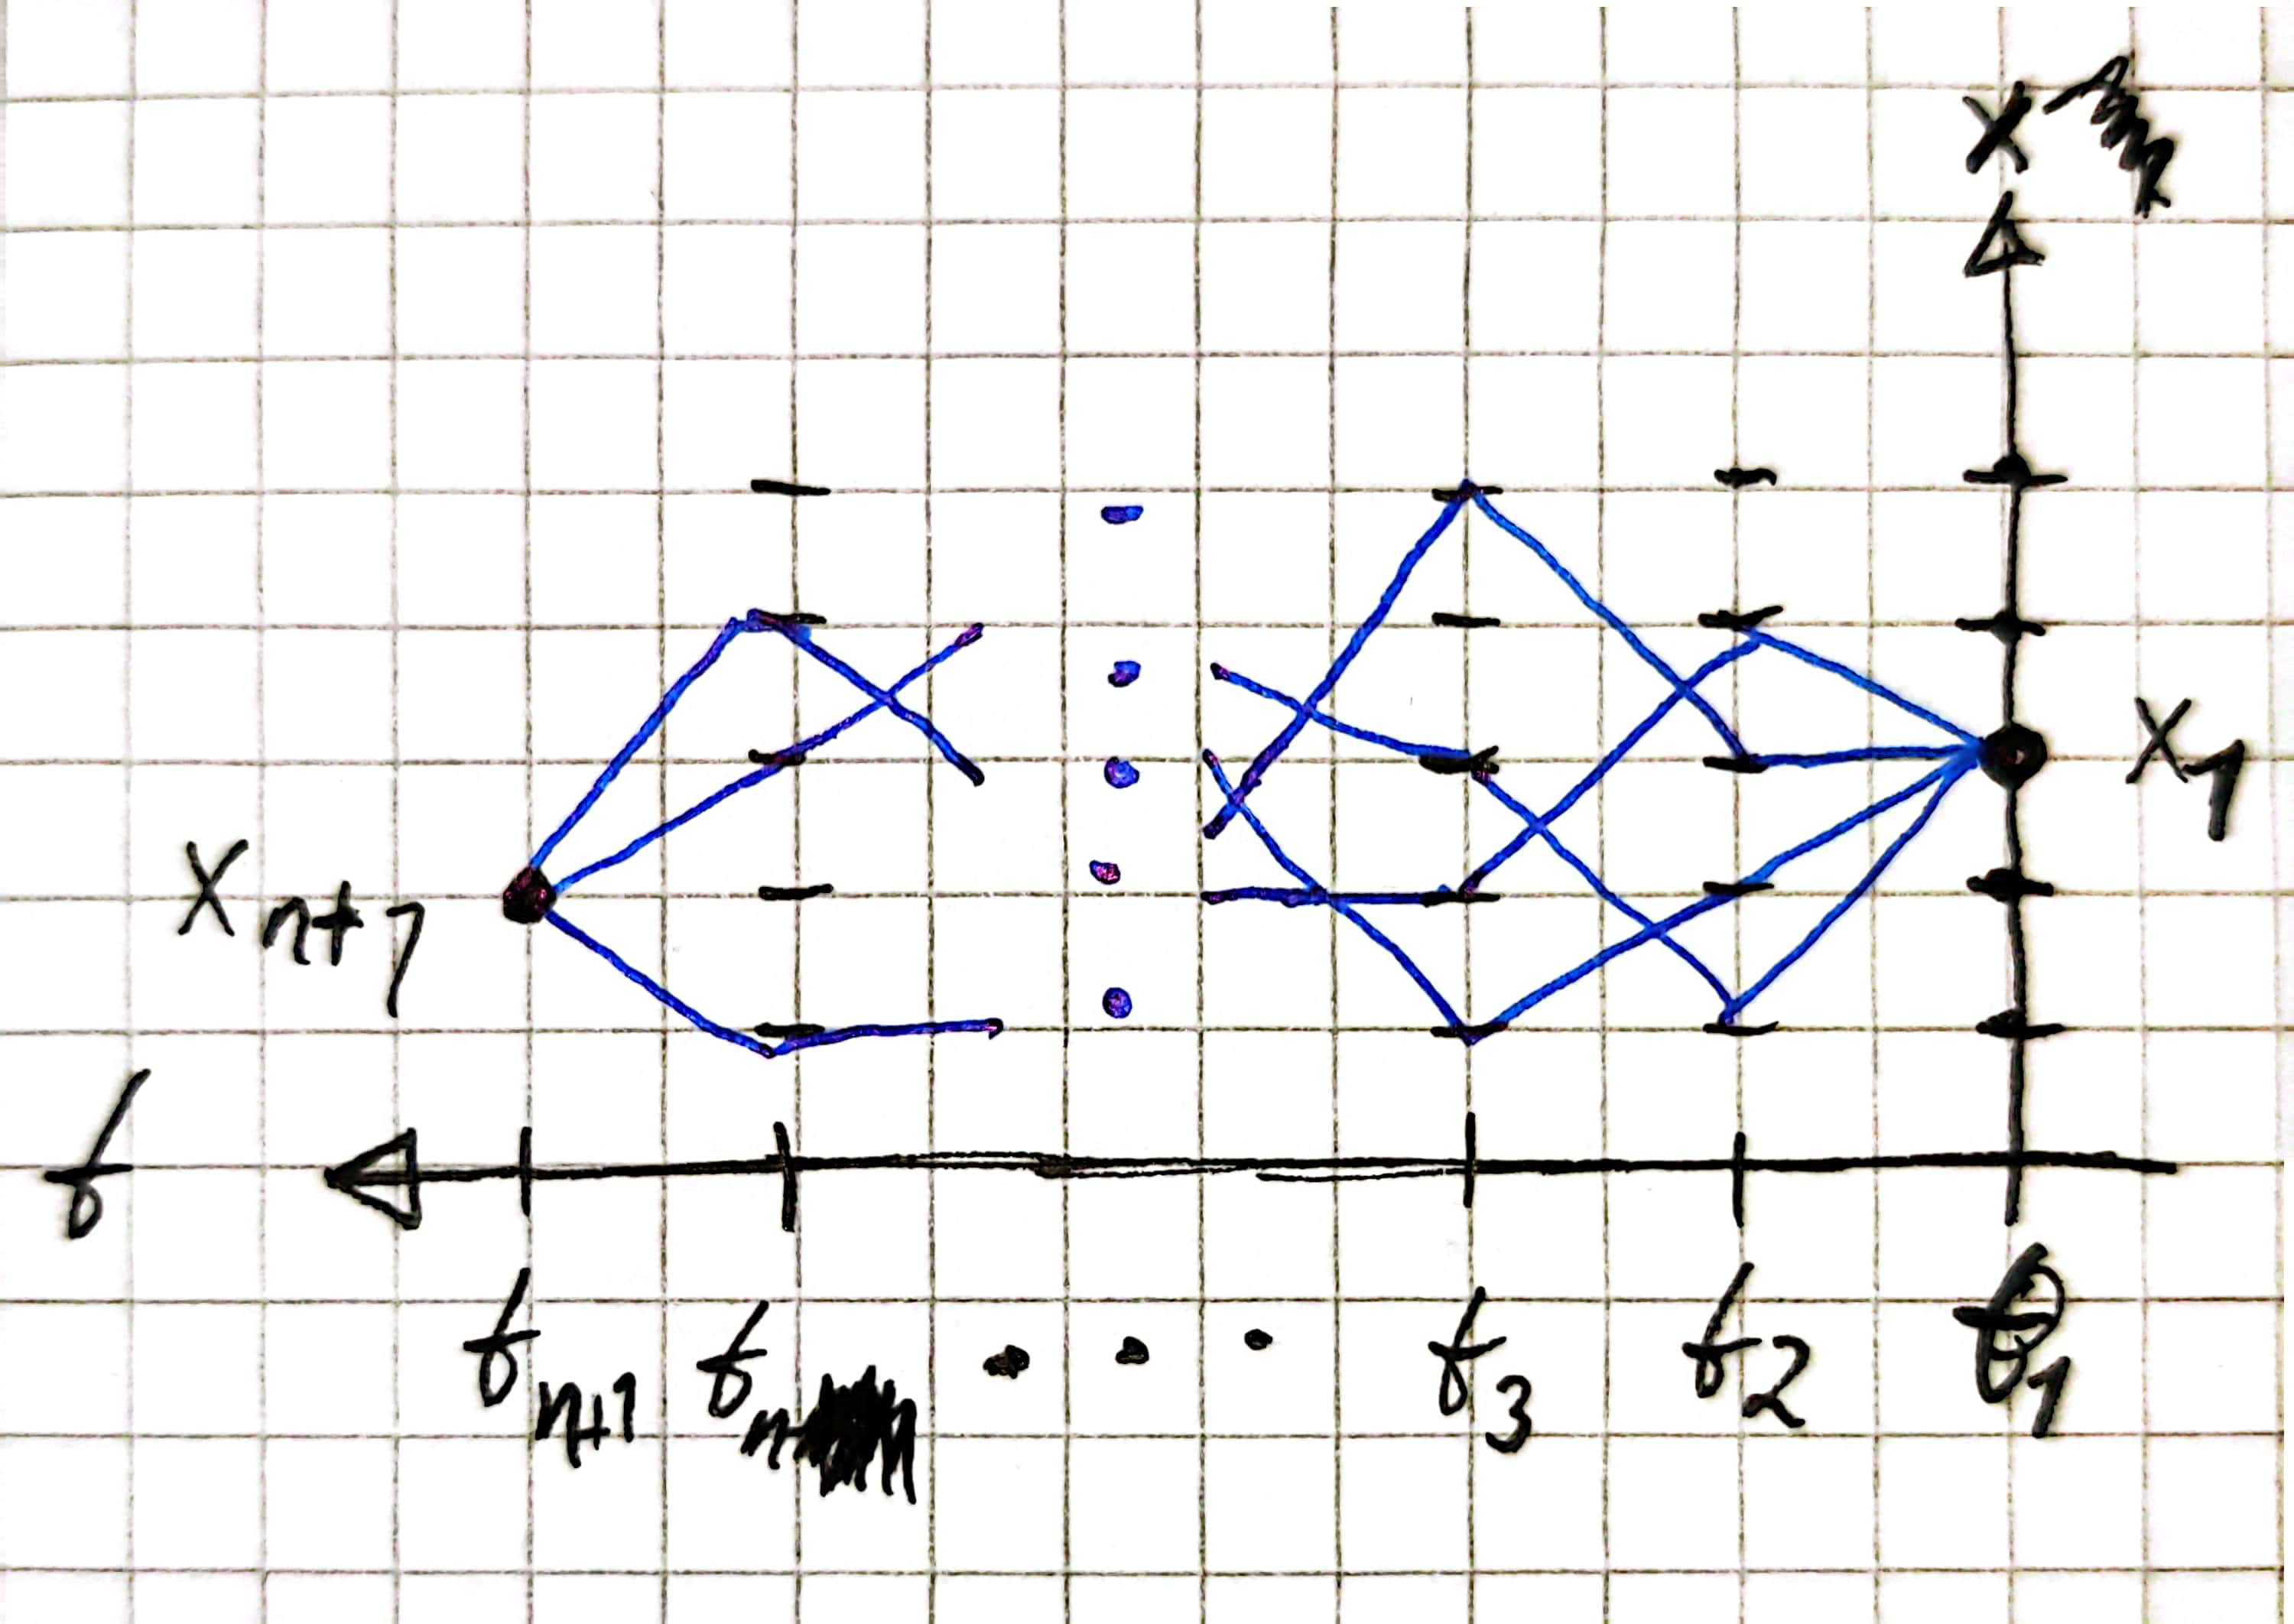
\includegraphics[width=.4\textwidth]{fig/fig2.jpg}
    \caption{Some of the paths between the initial and final state.}
    \label{fig: paths}
\end{figure}




\section{Gaussian process and the Ornstein-Uhlenbeck process}

The most important class of stochastic processes, as it is pretty much the only one we can solve, is Gaussian processes.
These have the form
%
\begin{align}
    P(x_{n+1}|x_n)
    =
    \frac{ 1 }{ \sqrt{ 2 \pi \sigma } }
    \exp \left\{ {-\frac{(x_{n+1} - \bar x_{n + 1})^2}{\sigma }} \right\}
\end{align}
%
Here, $\bar x_{n+1}$ is the expected value of $x_{n+1}$. \todo{Should there be som factors of $2$ here?}
As we consider Markovian processes, this is a function of only the previous step, $x_n$, and $\sigma$ is the variance of the process.


A specific example is the Ornstein-Uhlenbeck (OU) process,
%
\begin{align}
    \odv{ x(t) }{ t } = - \mu x(t) + \eta(t).
\end{align}
%
This models, for example, a particle on a spring in a fluid with thermal noise where friction dominates.
The $-\mu x(t)$ term is from Hooks law, and $\eta(t)$ is a random force modeling the forces of the fluid particles bumping into the particle.
You can read more about this process in~\footnote{\url{https://iopscience.iop.org/article/10.1088/1367-2630/ad7ef1/meta}}.
The expectation value of the OU-process at time $t_{n+1}$ is $x_n - \mu x_n \Delta t$---the where it was the step before minus the correction due to the spring-force.
The variance is $\sigma = \frac{2D}{\mu}(1  - e^{- 2 \mu \Delta t})$, where $D$ is the diffusion constant, which is the variance of the noise $\eta$.
With this, OU-process has the conditional probability distribution
%
\begin{align}
    P(x_{n + 1}| x_n) 
    = \sqrt{ \frac{ \mu }{ 4 \pi D \Delta t } }
    \exp \left\{ -
    \frac{ \left(x_{n + 1} - x_n + \mu x_n \Delta t\right)^2 }{ 4 D \Delta t } 
    \right\}
    = \sqrt{ \frac{ \mu }{ 4 \pi D \Delta t } }
    \exp \left\{ 
    - \frac{ \Delta t }{ 4 D }  \left(\dot x_{n + 1} + \mu x_n\right)^2
    \right\},
\end{align}
%
where we have introduced the discrete time-derivative, $\dot x_{n+1} = (x_{n + 1} - x_n) / \Delta t$.

We will now take two different limits, which will yield the path integral.
This means we will have to take the continuum limit.
If we consider the particles to live on a line instead of a lattice, then the position is given by a probability density $\Pe(x)$.
The probability of finding the particle between the points $x_i$ and $x_i + \Delta x$ is, for small $\Delta x$, $P(x) = P(x \in [x_i, x_i + \Delta x]) = \Pe(x) \Delta x$.
This allows us to go from sums to integrals,
%
\begin{align}
    \sum_{x} P(x) = \sum_{x} \Delta x \Pe(x) \underset{\Delta x \rightarrow 0}{\longrightarrow} \int \dd x \, \Pe(x).
\end{align}
%
Inserting the OU process into \autoref{eq: cond prob markov x0 given xn} and taking the continuous limit, we get
%
\begin{align}
    P(x_{n+1}|x_{1})
    & =
    \sum_{x_2\cdots x_{n+1}}
    \Delta x \Pe \left( x_{n+1}| x_{n} \right) \cdots \Delta x \Pe \left( x_{2}| x_{1} \right)\\
    &
    = \sum_{x_2\cdots x_{n+1}} \Delta x^n \exp \left\{ - \frac{\Delta t}{4 D} \sum_n \left[\dot x_{n + 1} - \mu x_n \right]^2 \right\}\\
    & 
    \underset{\substack{\Delta x \rightarrow 0\\ n \rightarrow \infty} }{ \sim }
    \int \D x(t) \,
    \exp \left\{ 
        - \frac{ 1 }{ 4D } 
        \int\limits_{t_1}^{t_{n+1}} \dd t \left[\dot x(t) + \mu x(t)\right]^2
        \right\}
    \equiv
    \int \D x(t) \, \Phi[x(t)].
\end{align}
%
$\Phi$ is the Onsager-Machlup \emph{functional}.
It is a functional, and not a function, as it takes in a function $x(t)$, and gives back a number.
We have defined the functional integration measure,
%
\begin{align}
    \D x(t) \equiv \lim_{\substack{\Delta x \rightarrow 0\\ n \rightarrow \infty} } \prod_{n} \Delta x \sqrt{ \frac{\mu}{ 4 \pi D \Delta t }}
\end{align}
%
This measure is not necessarily well-defined. 
To performed calculations, we will have re-descritize the path integral, so this can be considered as a notational trick rather than a true limit.


If we have a vector valued process instead, $\bm x(t) = x_a(t) \hat {\bm x}_a$, then the probability distribution is
%
\begin{align}
    P(x_{n_1}|x_n)
    = 
    \frac{ 1 }{ \sqrt{ 2 \pi \det \Sigma } }
    \exp \left\{ - \sum_{ab} (x_a(t_{n+1}) - \bar x_a(t_{n+1})) \Sigma_{ab}^{-1} (x_b(t_{n+1}) - \bar x_b(t_{n+1})) \right\}.
\end{align}
%
Here, $\Sigma$ is the covariance matrix of $x$.
An example of this may be a particle moving in three dimensions, so $\bm x$ is a three-dimensional vector, or a set of $N$ particles with position and velocity in three dimensions, so $\bm x$ is a $6 N$ component vector.


\section{Master equation}

We will here consider stochastic processes using a different formalism, the master equation.
If we consider a random process $N(t)$, and Taylor-expand the conditional probability of $N'$ at $t + \Delta t$ given $N$ at $t$ in small $\Delta t$, we get
%
\begin{align}\label{eq: expansion cond prob}
    P(N'(t + \Delta t)| N(t)) = 
    \underbrace{P(N'(t)|N(t))}_{\delta_{N'N}} + \Delta t 
    \underbrace{\pdv{P(N'(t')|N(t))}{t'}\bigg|_{t'=t}}_{W_t(N'|N)} + \Oh(\Delta t).
\end{align}
%
Here, we define the transition rates $W_t(N'|N)$.
This can be considered as a matrix, 
%
\begin{align}
    W_t(N'|N) = 
    \begin{pmatrix}
        W_t(1|1) & W_t(1|2)& W_t(1|3) &\cdots\\
        W_t(2|1) & W_t(2|2)& W_t(2|3) &\cdots \\
        \vdots & \vdots & \ddots & \cdots
    \end{pmatrix},
\end{align}
%
where the entries are the rate at which state $N'$ transitions to state $N$.
If we consider $N' = N$, then we can, by the principle of total probability (the probability of all possible outcomes add up to one), we can write
%
\begin{align}
    P(N(t + \Delta t)| N(t)) = 1 + \Delta t W_t(N|N) 
    = 1 - \sum_{N' \neq N}P(N'(t + \Delta t)| N(t))
    = 1 - \sum_{N' \neq N}\Delta t W_t(N',N),
\end{align}
%
or
%
\begin{align}\label{eq: rate cons condition}
    W_t(N|N) = - \sum_{N'\neq N}W_t(N'|N).
\end{align}
%
This insures the conservation of probability.
If we consider the matrix form of the rates, this means the diagonals of $W_t(N'|N)$ are given by minus the sum of each column,
\todo{is this right?}
%
\begin{align}
    W_t(N'|N) = 
    \begin{pmatrix}
        - \sum_{N\neq 1} W_t(N|1) & W_t(1|2)& W_t(1|3) &\cdots\\
        W_t(2|1) & - \sum_{N\neq 2} W_t(N|2)& W_t(2|3) &\cdots \\
        \vdots & \vdots & \ddots & \cdots
    \end{pmatrix},
\end{align}
%
If we expand the Chapman-Kolmogorov, \autoref{eq: chapman kolmogorov},
%
\begin{align}
    P(N(t_3) |N(t_1))
    & =
    \sum_{N(t_2)} 
    \left[
        \delta_{N(t_3)N(t_2)}
        + (t_3 - t_2) W_{t_2}(N(t_3)|N(t_2))
    \right]
    P(N(t_2)|N(t_1))
    \\
    & =
    (t_3 - t_2)\sum_{N(t_2)\neq N(t_3)} 
        W_{t_2}(N(t_3)|N(t_2)) P(N(t_2)|N(t_1))\\
    & \quad 
    + \left[ 1 + (t_3 - t_2) W_{t_2}(N(t_3)|N(t_2)=N(t_3))  \right] P(N(t_2)=N(t_3)|N(t_1))
\end{align}
%
If we apply \autoref{eq: rate cons condition}, and define $\Delta t = t_3 - t_2$, we can rearrange this to read
%
\begin{align}
    &\frac{P\left(N(t_3)|N(t_1)\right) - P(N(t_2)=N(t_3)|N(t_1))}{\Delta t}\\
    &=
    \sum_{N(t_2) \neq N(t_3)}
    \left[
        W_{t_2}(N(t_3)|N(t_2))P(N(t_2)|N(t_1))
        - W_{t_2}(N(t_2)|N(t_2)=N(t_3))P(N(t_2)=N(t_3)|N(t_1))
    \right]
\end{align}
%
The top line of this equation is the difference in probability of finding the system in the state $N(t_3)$ at time $t_3$ and $N(t_2)$, so in the limit $\Delta t \rightarrow 0$ becomes a derivative.
On the bottom, we have the diffenrence between the \emph{gain} rate and the \emph{loss} rate in to and out of state $N(t_3)$
We take the limit, which gives the \emph{master equation},
%
\begin{align}
    \odv{}{t} P(N(t)|N_0) =
    \sum_{N'\neq N} \left[
        W_t(N(t)|N'(t))P(N'(t)|N_0)
        - 
        W_t(N'(t)|N(t))P(N(t)|N_0)
    \right].
\end{align}
%
The master equation is equivalent to the Ornstein-Uhlenbeck path-integral---both are directly derived from the conditional probability distribution only by assuming the process is Markovian.
Although the two formulations are equivalent, they may be better or worse suited for different problems.

\begin{framed}
    \noindent
    \textbf{The quantum-stochastic analogy}\\
    The master-equation is first-order a linear ODE giving the time-evolution of a probability distribution.
    If this reminds you of the Schrödinger equation, the similarities does not stop here.
    In fact, the correspondence between the master-equation and the Onsager-Machlup functional is analogous to the relationship between the Schrödinger and the Feynman path integral in QM.
    The action of a process is a functional
    %
    \begin{align}
        S[x] = \int\limits_{t_a}^{t_b} \dd t \, L(x, \dot x, t), 
    \end{align}
    %
    where $L = V - T$ is the Lagrangian.
    In classical mechanics, the motion is determined by the Euler-Lagrange equations, $\fdv{ S }{ x(t) } = 0$, while in quantum-mechaics, the amplitude for a process is, according to the Feynman path integral,
    %
    \begin{align}
        K(x_a, x_b) &= \sum_{\mathrm{paths}\, x} \Phi[x], & \Phi[x] \propto e^{iS[x] / \hbar}.
    \end{align}
    %
    The Schrödinger equation gives the evolution of the wave-function,
    %
    \begin{align}
        i \hbar \odv{  }{ t } \Psi(x(t)) = \hat H \Psi(x(t)),
    \end{align}
    %
    where $\hat H$ is the Hamiltonian operator, and the amplitude is the overlap between the initial and finite wave-functions, $K(x_a, x_b) = \braket{ \Psi(x(t_b)) | \Psi(x(t_a)) } $.
\end{framed}




\section{Gaussian integrals}

The most important integrals we will meet are \emph{Gaussian integrals}.
The simplest Gaussian integral, which will be the basis for this chapter, is
%
\begin{align}\label{eq: gaussian integral}
    \int\limits_{-\infty}^\infty \dd x \, e^{-\frac{1}{2} a x^2} = \sqrt{ \frac{ 2 \pi  }{ a }}.
\end{align}
%
The reason we can solve Gaussian processes, as we mentioned earlier, is that we can solve Gaussian integrals.
With this simple result, we can solve path integrals over spaces of functions.
Consider
%
\begin{align}
    Z = \int \D \phi
    \exp \left\{ 
        - \frac{1}{2} \int \dd t_1 \dd t_2 \, 
        \sum_{ab}
        \phi_a(t_1) A_{ab}(t_1, t_2) \phi_b(t_2)
    \right\}.
\end{align}
%
Here, $\phi(t_1)$ is a vector function with $d$ components, $\phi_a(t) = (\phi_1(t), \phi_2(t)\dots)^T$, and $A_{ab}(t_1, t_2)$ is a matrix-function.
In the case of Markov-processes, $A(t_1, t_2)$ will be \emph{time-local}.
This means $A(t_1, t_2) = A(t_1) \delta(t_1 - t_2)$
For the path integral $Z$ to be well-defined, we must discretize $t_n = n \Delta t$, with $n \in \Z$
This gives us an extra set of indices, $\phi_a(t_i) = \phi_{a,i}$.
However, we can deal with this by ``unpacking'' the two-dimensional structure of $\phi_{a,i}$,
%
\begin{align}
    \phi_\alpha = 
    \left[\phi_1, ... \phi_N\right]
    =
    \left[
        \phi_{1, 1}, \phi_{2, 1}\dots\phi_{d,1}, \phi_{1, 2}\dots\phi_{d, n}
    \right],
\end{align}
%
where $N = d \times n$.
This is analogous to ``flattening'' an array in computer programming.
We also apply this to $A$.
The discretized dirac-delta is $\delta(t_1 - t_2) \sim \frac{1}{\Delta t} \delta_{t_1, t_2}$, so factoring out this $\Delta t$ we get 
%
\begin{align}
    A_{ab}(t_1,t_2)
    \sim \frac{1}{\Delta t} A_{ab,ij}
    \rightarrow \frac{1}{\Delta t} A_{\alpha \beta},
\end{align}
%
The path-internal then discretizes as 
%
\begin{align}
    Z = \int \left( \prod_{\alpha=1}^N \dd \phi_\alpha \right) \, 
    \exp \left\{ 
        \frac{1}{2} \Delta t \sum_{\alpha \beta} 
        \phi_\alpha A_{\alpha \beta} \phi_\beta
    \right\}.
\end{align}
%
We now assume $A$ is diagonalizable, so we can write it as $A = G \Lambda G^{-1} $, where $\Lambda = \mathrm{\lambda_1, ... \lambda_N}$ is diagonal, with $\lambda_\alpha$ are the eigenvalues of $A$.
We can therefore perform a change of variables, $z = G^{-1}\phi$, which simplifies the integral\todo{what about jacobian}
%
\begin{align}
    Z = \int \left( \prod_{\alpha=1}^N \dd z_\alpha \right)
    \exp \left\{ \frac{1}{2}\Delta t \sum_{\alpha} \lambda_\alpha z_\alpha^2 \right\}
    =
    \sqrt{ \det 2 \pi (\Delta t A)^{-1} }.
\end{align}
%
Here, we factored the exponential, used the simple Gaussian integral \autoref{eq: gaussian integral}, and used the fact that the product of the eigenvalues is the determinant.
